\section{Design}
\label{sec:design}


Our key design insight is that EFT and condition-number analysis require different numerical information but can share a unified shadow execution. Rather than executing two separate instrumentation pipelines, our design propagates a unified ShadowValue alongside every floating-point value. The shadow representation stores the information required by both analyses, allowing the pass to compute accumulated rounding error and numerical sensitivity simultaneously while avoiding duplicated instrumentation.

\subsection{System Overview}
\label{sec:system_overview}

Figure~\ref{fig:overview} illustrates the architecture of our LLVM instrumentation pass. During compilation, the pass rewrites floating-point operations to propagate a pass side ShadowValue for every floating-point value. Each ShadowValue maintains the information required by both the EFT-based error analysis and the condition-number analysis. During instrumentation, each floating-point SSA value is associated with a ShadowValue. The pass maintains a mapping between LLVM values and their corresponding shadow state, allowing subsequent instructions to reuse previously computed metadata. When the program executes, this metadata is converted to a runtime ShadowEntry to preserve state across memory operations and function calls. The runtime debugger then consumes the propagated shadow state to detect excessive rounding error, cancellation, sensitivity, branch divergence, and non-finite results.

\begin{figure}[t]
\centering
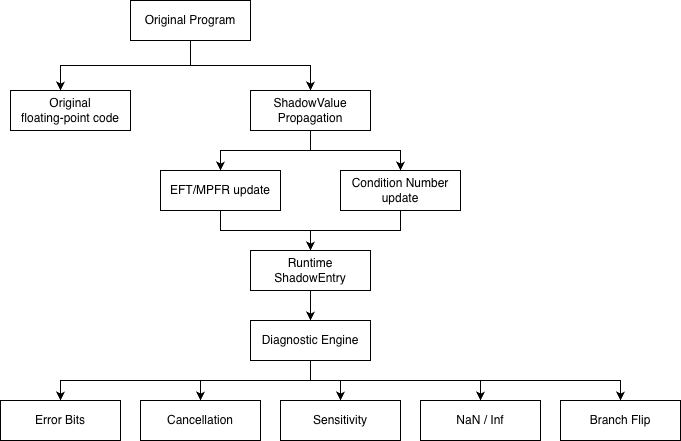
\includegraphics[width=0.75\columnwidth]{figures/overview.png}
\caption{Architecture of the analysis framework. The LLVM pass propagates unified shadow state through EFT/MPFR error tracking and condition-number analysis, while runtime shadow memory preserves metadata across memory and function boundaries. Diagnostic engine uses the propagated shadow states to report numerical errors.}
\label{fig:overview}
\end{figure}

\subsection{Instrumentation}
\label{sec:instrumentation}

\subsubsection{Shadow Representation}
\label{sec:shadowvalue}
Each floating-point SSA value is associated with a pass-side \texttt{ShadowValue} containing the metadata required to propagate both analyses. LLVM IR follows static single assignment (SSA) form, where each instruction produces a unique value. This property naturally enables shadow propagation because every floating-point result has exactly one corresponding ShadowValue. Each floating-point SSA value is recorded by the instrumentation to a local value map. Before constructing a new one, the pass first checks if a ShadowValue is already generated. Reusing stored values prevents duplicated generation and ensures that instructions with the same SSA value will get same propagated error state. When an instruction produces a new result, its ShadowValue is updated and inserted into the map. 
\[
[\hat{x}, \hat{r}, \texttt{s}, \hat{e}, \texttt{i}, \texttt{R}]
\]
A ShadowValue stores six pieces of information. The pair ($\hat{x}, \hat{r}$) represents the computed value and its accumulated error. The sign bit $s$, exponent estimate $\hat{e}$, compile-time exact flag $i$, and propagated relative error $R$ provide the information required by condition-number propagation and runtime diagnostics.
The runtime representation, \texttt{ShadowEntry}, uses this metadata in runtime for across memory operations and function boundaries. Runtime ShadowEntries are stored in the shadow table for memory access and moved to shadow stack across function calls.

\subsubsection{Memory Shadowing}
\label{sec:memory_shadowing}
SSA-based shadow propagation is insufficient when floating-point values are written to memory and later reloaded. To preserve metadata across those operations, the runtime maintains a shadow table indexed by application memory address. A \texttt{store} writes the value's shadow entry to the corresponding shadow address, while a \texttt{load} retrieves the previously stored metadata and associates it with the newly created LLVM SSA value. This connects compile-time propagation with runtime propagation. Figure~\ref{fig:memory} shows how pass side ShadowValue and runtime side ShadowEntry is stored and loaded.

\begin{figure}[t]
\centering
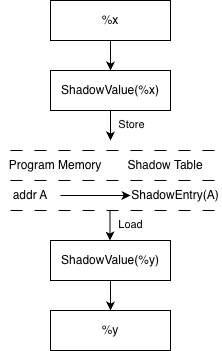
\includegraphics[width=0.5\columnwidth]{figures/memory.png}
\caption{Shadow-state propagation across memory operations. A store converts pass-side ShadowValue to a runtime ShadowEntry indexed by the application address; a load restores the metadata for the newly loaded SSA value.}
\label{fig:memory}
\end{figure}

\subsubsection{Function-Boundary State}
\label{sec:memory_call_boundary}
Function calls introduce another boundary as LLVM arguments and return values are represented by different SSA values in the caller and callee. This prevents metadata transfer through the pass-side value map, which is why runtime maintains a shadow stack. The runtime shadow stack transfers metadata for floating-point arguments into the callee and carries the return-value metadata back to the caller. This preserves the error state across function boundaries without changing the program's original calling convention. Figure~\ref{fig:function_call} shows how the caller and callee retrieves shadow state.

\begin{figure}[t]
\centering
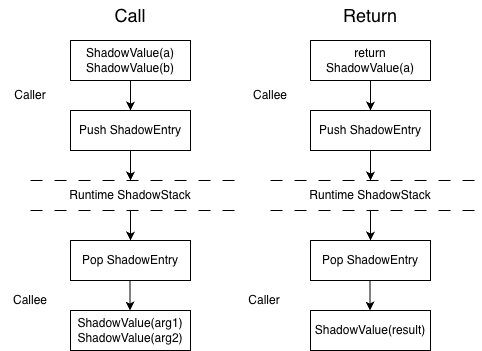
\includegraphics[width=0.7\columnwidth]{figures/function_call.png}
\caption{Shadow-state propagation across function boundaries. Argument metadata is transferred from caller to callee through the runtime shadow stack, with the corresponding mechanism used to propagate return-value metadata back to the caller.}
\label{fig:function_call}
\end{figure}

\subsection{Error Propagation}
\label{sec:error_propagation}
Shadow propagation computes how numerical error evolves throughout program execution. Each floating-point instruction updates the associated ShadowValue by propagating both accumulated rounding error and relative error to the result. 

\subsubsection{Error-Free Transformation}
\label{sec:eft}
For primitive arithmetic operations (\texttt{FAdd}, \texttt{FSub}, \texttt{FMul}, \texttt{FDiv}, and \texttt{Sqrt}), the pass computes each operation using an Error-Free Transformation (EFT). Unlike conventional floating-point arithmetic, an EFT computes both the rounded result $\hat{x}$ and its associated rounding residual $\hat{r}$ so their sum exactly represents the real-valued result.\\
Because these transformations are expressed entirely with hardware-supported floating-point operations (e.g., \texttt{TwoSum} and \texttt{FMA}), they are emitted directly into the LLVM IR instead of being implemented as runtime library calls. Inlining these transformations eliminates the overhead of invoking the runtime for every arithmetic instruction while preserving exact residual computation. The computed residual is then accumulated into the ShadowValue and propagated to subsequent floating-point operations. Figure~\ref{fig:error_prop} shows how a sample LLVM IR is instrumented.

\begin{figure}[t]
\centering
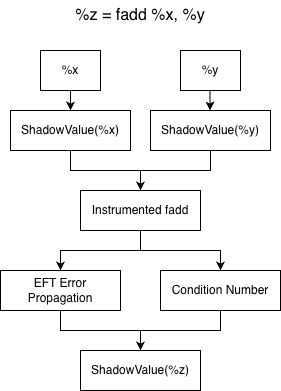
\includegraphics[width=0.5\columnwidth]{figures/error_prop.png}
\caption{Instrumentation of a floating-point operation. Operand ShadowValues are retrieved for the original SSA operands, updated by EFT error propagation and condition-number analysis, and generate the resulting SSA value.}
\label{fig:error_prop}
\end{figure}

\subsubsection{MPFR}
\label{sec:mpfr}
Not all floating-point operations have efficient Error-Free Transformations. In particular, transcendental functions such as \texttt{sin}, \texttt{cos}, \texttt{exp}, and \texttt{log} require a different propagation strategy. For these operations, the pass inserts runtime calls to handlers implemented using the MPFR multiple-precision library.\\
Each runtime handler evaluates the mathematical function at higher precision to approximate the exact result while simultaneously propagating the incoming error using a first-order Taylor expansion. If the input is represented as $a+\delta a$, the propagated error is approximated as
\[
f(a+\delta a)
\approx
f(a)+f'(a)\delta a
\]
The resulting absolute error is stored in the propagated ShadowValue, allowing transcendental functions to participate in the same analysis pipeline as primitive arithmetic operations.

\subsection{Condition Number Analysis}
\label{sec:condition_number}
While EFT accurately measures accumulated rounding error, it does not capture the numerical sensitivity of an operation. A computation may exhibit a very small rounding residual while remaining highly sensitive to perturbations in its inputs. To distinguish these cases, our analysis propagates a relative error estimate based on condition numbers alongside the EFT residual.\\
We reuse the operation-specific split factors and condition-number propagation rules introduced by  ExplainiFloat~\cite{explainifloat}. Our contribution is not a new condition-number formulation but the integration of condition number propagation with an independently propagated EFT/MPFR residual in a single dynamic analysis over shadow state.


The two signals serve different roles. EFT and MPFR estimate the error that has actually accumulated along the observed execution, whereas the condition-number state estimates how strongly an operation amplifies perturbations in its operands. Our diagnostic policy evaluates these signals together: the propagated error determines whether the observed result is inaccurate, while the split factors identify whether the instability is attributable to cancellation or sensitivity. This combined decision procedure avoids treating all large EFT residuals as the same error category and avoids reporting numerical sensitivity when it doesn't produce a meaningful error in the observed execution.

ExplainiFloat, which uses a logarithmic-number system oracle and reports a 4.24$\times$ speedup over arbritrary-precision arithmetic~\cite{explainifloat}. We instead reuse the EFT residual already required for error tracking, avoiding a second oracle entirely, at the cost of dynamic-range saturation discussed in \ref{sec:disc_sensitivity}.

\subsection{Diagnostic Generation}
\label{sec:diagnostic}
The diagnostic engine converts propagated shadow state into user-visible numerical error reports. Rather than treating all numerical failures as a single category, the debugger combines the accumulated error tracked by EFT/MPFR with the classification produced by condition-number analysis.\\
Error-magnitude detection compares the computed floating-point result against the corrected value reconstructed from its propagated error and reports cases exceeding a configurable bit-error threshold. NaN and infinity are detected separately as non-finite results. Condition-number detections classify numerically unstable operations as cancellation or sensitivity. The debugger additionally checks numerical effects that can alter program semantics: conversions are reevaluated using the corrected value, and floating-point branch predicates are reevaluated using corrected operands to identify potential branch divergences.

% \begin{figure}[t]
% \centering
% 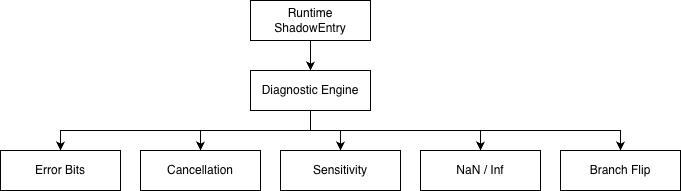
\includegraphics[width=0.5\columnwidth]{figures/dignostics.png}
% \caption{Diagnostic generation from propagated shadow state. The runtime diagnostic engine combines accumulated error information and condition-number classification to report error magnitude, non-finite values, numerical instability, conversion errors, and control-flow divergence.}
% \label{fig:diagnostics}
% \end{figure}

